\chapter{Resultat}

\begin{wrapfigure}{r}{0.7\textwidth}
    \centering
    \vspace{-40pt}
    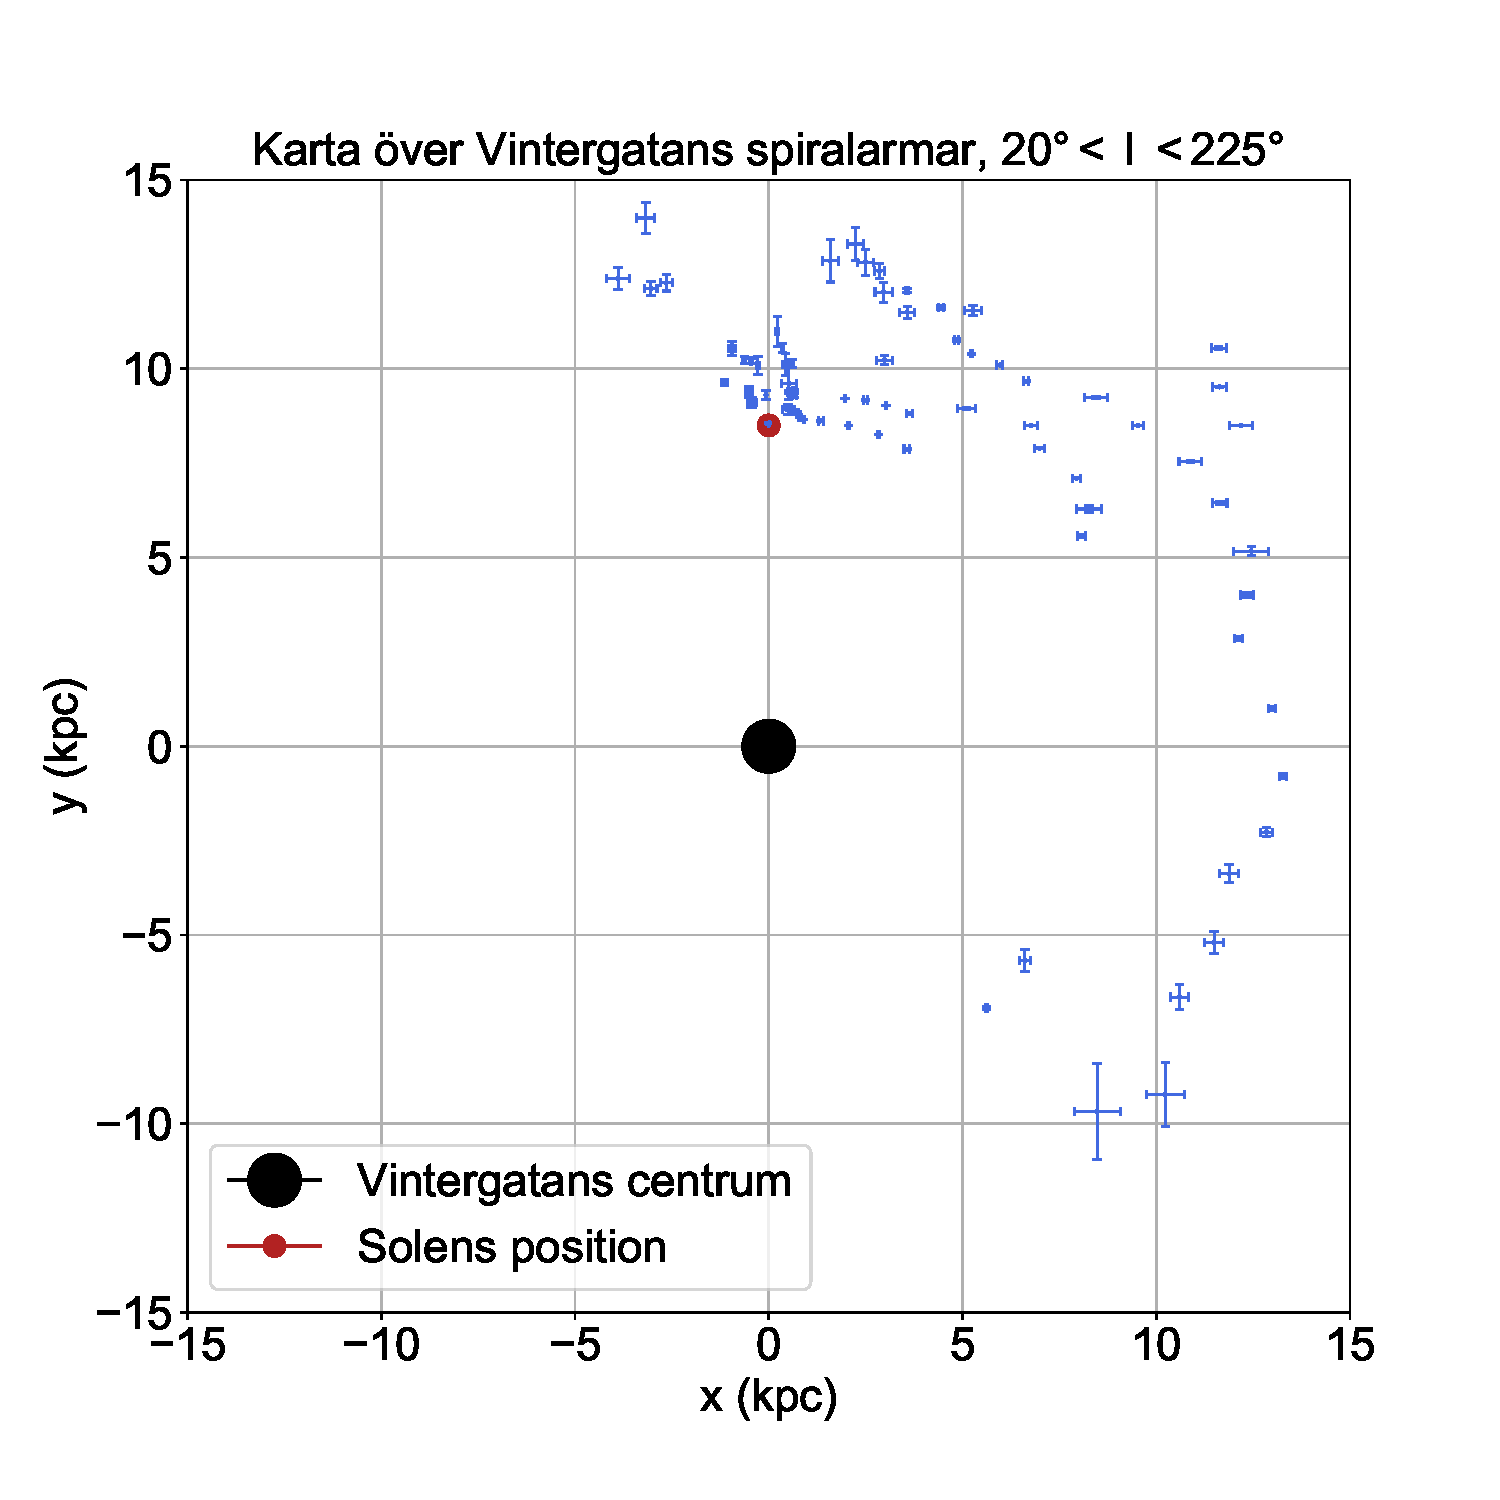
\includegraphics[max size={0.7\textwidth}{\textheight}]{pics/GustavVilhelm.pdf}
    %\vspace{20pt}
    \caption{Vår karta över Vintergatan}
    \label{fig:map_our}
\end{wrapfigure}

För varje mätning har vi nu två möjliga värden på r, avståndet mellan molnet och Vintergatans centrum. Om det ena värdet på r är negativt förkastar vi det och använder det positiva värdet som det ''riktiga'' värdet på r, men i det fall vi fick två positiva lösningar förkastade vi båda.

Utifrån de resulterande värdena ritade vi upp en karta över varje mätning, se figur \ref{fig:map_our}. Våra mätvärden och uträkningar återfinns i bilaga 1.